\section{Temperature Acquisition Channel}

	\subsection{Thermocouple Type and Signal}	
			
	 For this project it was defined that thermocouples of type K (formed by the junction of two metal leagues: Alumel and Cromel) would be used in this project. This is because this specific type of thermocouple has a wide range of operation (-200$^{\circ}$C - 1200 $^{\circ}$C), so according to the requirements they are never too close from the boundary values, a thermocouple of type T or even a type J would not be suitable. Other appealing factor is that this type of thermocouple is quite common so getting eventual replacements would be easier, in comparisson with type E thermocouples.

	\subsection{Thermocouple Signal Conditioning}
	
	As mentioned in sub-section \ref{ssec:thermocouple}, besides amplification and linearization, the thermocouple signal also needs it's cold junction temperature difference compensation. There is an integrated solution from \textit{Analog Device} called AD8495, this IC functional diagram is displayed on Figure \ref{fig:ad8495-functional-block}.
	
		\begin{figure}[htbp]
			\centering
				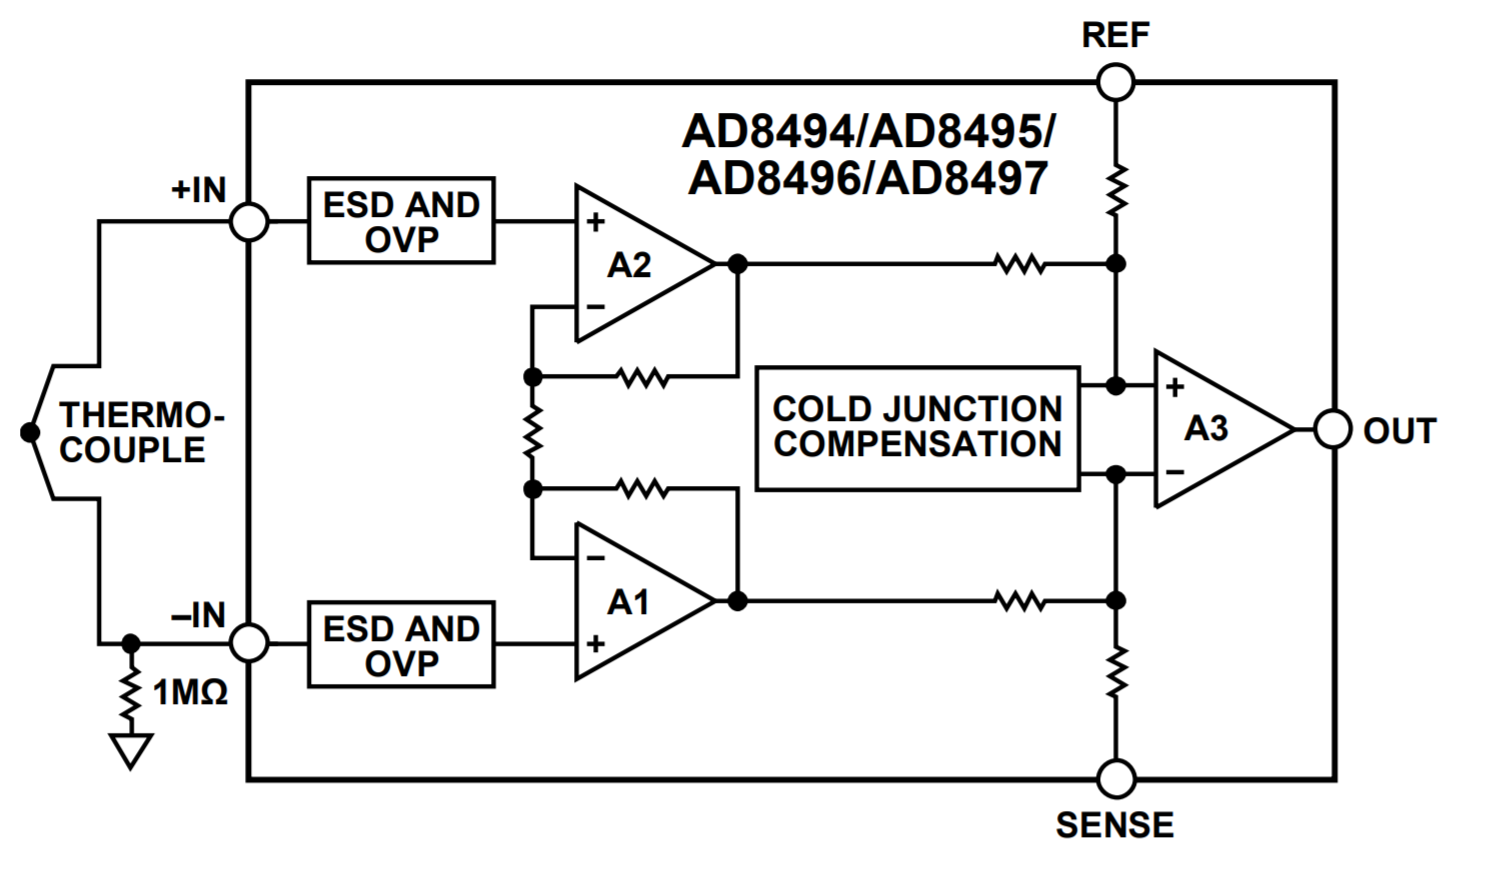
\includegraphics[scale=0.65]{figuras/fig-ad8495-functional-block}
			\caption{AD8495 Functional Block Diagram \cite{ad8495-functional-block}}
			\label{fig:ad8495-functional-block}
		\end{figure}
		
	This IC produces a linearized output with a fixed gain of $5mv\/^\circ}$C, it is a quite practical solution as it can be powered with single-supply voltage source and it's output saturates to the power supply voltage if the thermocouple is disconnected \cite{ad8495-datasheet}.
	
	\subsection{Input Protection and Filtering}\label{ssec:ad8495InputProtectionAndFiltering}
	
	Although this IC already has overvoltage and ESD protection, thermocouples tips can pick a load of unwanted noise and transients. Hence, additional protection and external filtering is also recommended by \cite{two-ways-thermocouple}. First thing to do is to add current-limint series resistors, the drawback is doing that is that resistors in the circuit net increases the overall noise. This type of noise is called Johnson-Nyquist Thermal Noise or more commonly just by Johnson Noise, thermal agitation of electrons in a resistor gives rise to random fluctuations in the voltage across its terminals \cite{romero1998johnson}. Moreover, it can be calculated using the following Equation \ref{eqn:johnson-noise} where K is the Boltzamann's constant $1.38 \cdot 10^{-23}$, R is the resistance in ohms $(\Omega)$ and T the temperature in kelvin (~300K at room temperature) \cite{sensors2000}.
	
		\begin{equation}\label{eqn:johnson-noise}
			Noise (nv\/\sqrt{Hz}) = \sqrt{4 \cdot K \cdot R \cdot T \cdot 10^{9}}
		\end{equation}
		
	Because the protection circuit includes two equal resistors, whose noise is uncorrelated, that is, the two noise sources are independent of each other—the above result must be multiplied by the square root of 2 (the root sum square of the two noise voltages) and it is considered as a general rule design to tolerate additional Johnson Noise from 10 to 30$\%$ to the amplifier IC \cite{sensors2000}. \cite{two-ways-thermocouple} suggests using current-limiting resistors of 10$k\Omega$, according to the AD8495 datasheet \cite{ad8495-datasheet}, the choosen amplifier (AD8495) has a voltage noise density of 32nV$\/ \sqrt{Hz}$. Combining this resistors noise with the amplifier noise will produce a overall noise of 36.85nV$\/\sqrt{Hz}$, which is just 13$\%$ above the amplifier's own noise. Additional protection can be achieved using external protection diodes as on Figure \ref{fig:externalProtectionDiodes}.
	
		\begin{figure}[htbp]
			\centering
				\includegraphics[scale=0.65]{figuras/fig-externalProtectionDiodes}
			\caption{External Protection Diodes \cite{externalProtectionDiodes}}
			\label{fig:externalProtectionDiodes}
		\end{figure}
		
	A Transient Voltage Suppression Diode (TVS) can be used to protect the inputs from differential input overvoltage, considering a bidirectional TVS with a 5V breakdown voltage, the device will theoretically limit the differential voltage between 5V and -5V, the AD8495 has overvoltage protection from -25V to 20V when powered with 5V, so this will successfully protect the amplifier inputs. It is also interesting to clamp each input to the supply rails using, this is best done using Schottky diodes, this type of diode operates the same way as standard diodes but have faster response and lower forward voltage. Schottky diodes have a foward voltage of approximately 200mV, if the supply rails are of 5V and 0V, a pair of diodes connected in the same way of Figure \ref{fig:externalProtectionDiodes}, the inputs will be clamped on -200mV and 5200mV, protecting the input.
	\par
	With the overloads protection done, another important feature to do is to filter unwanted signals in the inputs to avoid them to be amplified later, this is done by filtering Radio Frequency Interference (RFI), signal lines (specially for low level signals) are quite susceptible to RF interference \cite{analogDevDesignersGuide}. Interference that occurs on both lines are usually reduced by the amplifiers own common-mode rejection filter, but only on a limited bandwidth, also the in-amp rectifier cannot filter differential RF interference. The choosen amplifier (AD8495) has a -3dB bandwidth at 25kHz, \cite{two-ways-thermocouple} suggests setting a common-mode cutoff filter frequency at 16kHz (in order to guarantee the input signal within the 25kHz bandwidth). The standard circuit for the RFI filter is displayed on Figure \ref{fig:rfi-standard-filter}, resistors R1 and capacitors C1 are used to filter common-mode interference and it is important that state that $R1_{a}$=$R1_{b}$ and $C1_{a}$=$C1_{b}$. Capacitor C2 is connected across the bridge output to reduce any common-mode rejection errors due to the components mismatch, that way filtering any differential interference. C2 is usually choosen to be ten times larger than C1 \cite{ad8495-datasheet}.
	
		\begin{figure}[htbp]
			\centering
				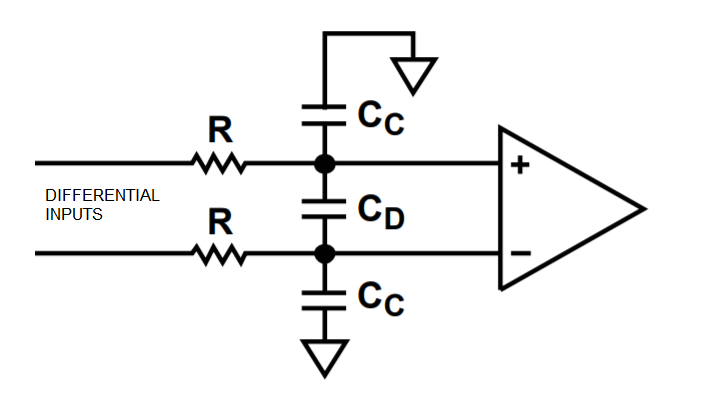
\includegraphics[scale=0.65]{figuras/fig-rfi-standard-filter}
			\caption{RFI filter circuit \cite{fig-rfi-standard-filter}}
			\label{fig:rfi-standard-filter}
		\end{figure}

	The -3dB common-mode bandwidth of this filter from Figure \ref{fig:rfi-standard-filter} is given by Equation \ref{eqn:bw-common-mode-rejection-filter} \cite{analogDevDesignersGuide}.

		\begin{equation}\label{eqn:bw-common-mode-rejection-filter}
			BW_{CM}=\frac{1}{2 \cdot \pi \cdot R1 \cdot C1}
		\end{equation}
	
	The -3dB differential bandwidth of this filter from Figure \ref{fig:rfi-standard-filter} is given by Equation \ref{eqn:bw-differential-rejection-filter} \cite{analogDevDesignersGuide}.
	
		\begin{equation}\label{eqn:bw-differential-rejection-filter}
			BW_{DIFF}=\frac{1}{2 \cdot \pi \cdot R1 \cdot \left( 2 \cdot C2 + C1 \right)}
		\end{equation}
		
	Using the values for the current limiting resistors (10k$\Omega$), Equation \ref{eqn:bw-common-mode-rejection-filter} and the suggested cutoff frequency of 16kHz \cite{two-ways-thermocouple}, it is possible to calculate a value of 1nF for C1. Choosing a C2 value ten times larger than C1 implies on using a C2 value of 10nF, that used on Equation \ref{eqn:bw-differential-rejection-filter} will produce a differential interference filter cutoff frequency of 1.3kHz.
		
	\subsection{Thermocouple Sensor Detection}
		
	A important feature of any acquisition system is to detect when a sensor is disconnected from the the acquisition system input \cite{o2011pressure}, because a signal acquisition circuit without the signal source will generate outputs that are uncorrelated to what the system was designed to measure/sense on the outside world. The AD8495 has a quite useful feature \cite{ad8495-datasheet}, it offers open thermocouple detection, the inputs of the AD8495 are PNP type transistors, which means that the bias current always flows out of the inputs. This way, the input bias current drives any unconnected output high, which saturates the output to the maximum possible reading, being in this case 1000$^{o}$C or 5V (considering the fixed 5mv$\/ ^{o}$C gain. In Section \ref{sec:functionalRequirements}, it was defined that the system must measure temperatures up to 600$^{o}$C, with the fixed gain of 5mv$\/^{o}$ this means an output voltage of 3V. So the so called \textit{Thermocouple Sensor Detection} must be able to detect whenever the output exceeds 3V. In order to do that, the circuit displayed in Figure \ref{fig:thermocouple-sensor-detection} was designed.
	
		\begin{figure}[htbp]
			\centering
				\includegraphics[scale=0.65]{figuras/fig-thermocouple-sensor-detection}
			\caption{Thermocouple Sensor Detection Circuit}
			\label{fig:thermocouple-sensor-detection}
		\end{figure}
		
	The diode D1 is a 3V9 zener diode, added this with the transistor Q1 (BC548) which has a typical \textit{Base-Emitter On Voltage} of 660mV \cite{bc548 }, whenever the input voltage (AD8495 output voltage) exceeds 4.56V, it will turn Q1 on. When Q1 is on the output will be the 5V from the source, when Q1 is off (voltage not exceeding the 4.56V threshold) the \textit{pull-down} resistor at Q1 emitter will take the output voltage to 0V meaning there is no disconnection issue. The other 10k$\Omega$ resistor is a \textit{pull-down} used to guarantee that the base-emitter voltage is 0V if there is no voltage on the AD8495 output. The 4.7k$\Omega$ resistor is a current limiting resistor used just to make sure just a small amount of current will be driven from the AD8495 output.

	\substion{Final Circuit}
	
